\documentclass[12pt, t]{beamer}
\usepackage{graphicx}
\usepackage{amsmath}
\usepackage{setspace}
\usepackage{float} 
\usepackage{multido}
\usepackage{multirow}
\usepackage{array}
\usepackage{enumerate}
\usepackage{booktabs}
\usepackage{indentfirst} 
\usepackage[style=mla]{biblatex}
\usepackage{subcaption}
\usepackage{hyperref}
\usepackage{textpos}
\usepackage{mathtools, nccmath}
\usepackage{listings}
\usepackage{animate}

\colorlet{mygray}{black!30}
\colorlet{mygreen}{green!60!blue}
\colorlet{mymauve}{red!60!blue}

\lstset{
  basicstyle=\fontsize{9}{10}\ttfamily,
  columns=fullflexible,
  breakatwhitespace=false,      
  breaklines=true,                
  captionpos=b,                    
  commentstyle=\color{mygreen}, 
  extendedchars=true,              
  frame=single,                   
  keepspaces=true,             
  keywordstyle=\color{blue},      
  language=c++,                 
  numbers=none,                
  numbersep=5pt,                   
  numberstyle=\tiny\color{blue}, 
  rulecolor=\color{mygray},        
  showspaces=false,               
  showtabs=false,                 
  stepnumber=5,                  
  stringstyle=\color{mymauve},    
  tabsize=3,                      
  title=\lstname                
}

\makeatletter
\let\@@magyar@captionfix\relax
\makeatother

\definecolor{Turquoise3}{RGB}{0, 134, 139}
\renewcommand{\emph}[1]{{\color{Turquoise3}\textsl{#1}}}
\newcommand{\C}{\mathbb{C}} \newcommand{\F}{\mathbb{F}} \newcommand{\R}{\mathbb{R}} \newcommand{\Q}{\mathbb{Q}}
\newcommand{\N}{\mathbb{N}}
\newcommand{\myseries}[2]{$#1_1,#1_2,\dots,#1_#2$}
\newcommand{\nullspace}{~\\[15pt]}
\newcommand{\remark}{\textbf{Remark: }}
\newcommand{\scp}[2]{\langle\,#1\,,\,#2\,\rangle} \newcommand{\scpp}{\langle\,\cdot\,,\,\cdot\,\rangle}


\usetheme{Madrid}
\setbeamertemplate{navigation symbols}{}

\addtobeamertemplate{frametitle}{}{
\begin{textblock*}{100mm}(0.85\textwidth,-1cm)

\includegraphics[height=1cm]{Figures/logo/logo.png}
\end{textblock*}}

\definecolor{themecolor}{RGB}{25,25,112} 

\usecolortheme[named=themecolor]{structure}

\setbeamertemplate{items}[default]

\hypersetup{
    colorlinks=true,
    linkcolor=themecolor,
    filecolor=themecolor,      
    urlcolor=themecolor,
    citecolor=themecolor,
}

\title{Vv214 Final Project}
\subtitle{\textbf{Donut.c}}
\institute[UM-SJTU JI]{University of Michigan-Shanghai Jiao Tong University Joint Institute}
\author{Pingbang Hu, Xiaoyu Chen, Jinyi Wu}

\begin{document}

\begin{frame}
    \titlepage
    \begin{center}
        
\includegraphics[height=2cm]{Figures/logo/logo2.png}
    \end{center}
\end{frame}

%--------------------------------------------------------------------------------------------------
\section{Overview}
    \begin{frame}
        \frametitle{Overview}
        \begin{enumerate}
            \item Motivation
            \item Introduction
            \item Draw a donut
            \item Rotate a donut
            \item Bright and dark
            \item Projection into terminal
            \item Discrete Dynamic System
            \item Demonstration
            \item Source Code
            \item Reference
        \end{enumerate}
    \end{frame}

%--------------------------------------------------------------------------------------------------

\section{Motivation}
\begin{frame}
    \frametitle{Motivation}

    Back in 2006, there's an interesting c project called Donut.c, which will print a rotating 
    donut in the terminal.

    \nullspace
    Looking into the source code and a blog updated recently by the author, we find out 
    that this program is highly depended on what we have learned in Vv214.

    \nullspace
    After some discussion, we decide to dive into the source code and analyze the whole mechanism 
    behind it.

\end{frame}

%--------------------------------------------------------------------------------------------------

\section{Introduction}
\begin{frame}
    \frametitle{Introduction}

    To start with, we first need to design a way to show the donut. Since the terminal has a dark 
    background with white character.
    
    \nullspace
    We let the \textbf{size} of the character to mimic the brightness of a single pixel. We show 
    the character array as below, from the darkest to the brightest:

    \begin{equation*}
        \{.\quad ,\quad -~\quad ;\quad =\quad !\quad *\quad \#\quad \$\quad @\}
    \end{equation*}

    \nullspace
    With these characters, we can generate some black \& white \emph{ascii art} in the terminal!

\end{frame}

%--------------------------------------------------------------------------------------------------

\section{Draw a donut}
\begin{frame}
    \frametitle{Draw a donut}

    Now we have the way to show some diagrams in the terminal, then we start to consider how to 
    actually generate a rotating donut in the terminal.

    \nullspace
    In a mathematical way to produce a donut, we start with the concept of \emph{parametric equation}.
    Since a donut basically is a circle rotating respected to the axis parallel to the fixed diameter,
    with some simply geometry, we have:

    \begin{equation*}
        \begin{pmatrix}
            x   \\
            y   \\
            z
        \end{pmatrix}
        =
        \begin{pmatrix}
            R_2 \\
            0   \\
            0
        \end{pmatrix}
        +
        \begin{pmatrix}
            R_1\cos{\theta} \\
            R_1\sin{\theta} \\
            0
        \end{pmatrix}
        ,\quad \theta \in [0,2\pi)
    \end{equation*}

    which produce two circles in the $x-y$ plane.

\end{frame}

%--------------------------------------------------------------------------------------------------

\section{Draw a donut}
\begin{frame}
    \frametitle{Draw a donut}

    Since we now have two circles, we now only need to rotate these circles for $\pi$ degree by 
    applying a \emph{rotation matrix w.r.t. y-axis}.

    \nullspace
    With the parametric equation we have derived, we have:

    \begin{equation*}
        \underbrace{
        \begin{pmatrix}
            \cos\phi & 0 & \sin\phi \\
            0 & 1 & 0\\
            -\sin\phi & 0 & \cos\phi
        \end{pmatrix}
        }_\text{Y : rotation matrix for y-axis}
        \cdot
        \underbrace{
            \begin{pmatrix}
                R_2 + R_1\cos{\theta} \\
                R_1\sin{\theta} \\
                0
            \end{pmatrix}
        }_\text{two circles' parametric eqs.}
        ,\quad
        \begin{cases}
            \theta \in [0,2\pi)\\
            \phi   \in [0,\pi)
        \end{cases}
    \end{equation*}

    \nullspace
    This produce a full donut in the 3 dimensional space. And for simplicity, we will now omit 
    the angles' ranges from now on. 

\end{frame}

%--------------------------------------------------------------------------------------------------

\section{Draw a donut}
\begin{frame}
    \frametitle{Draw a donut}

    \animategraphics[autoplay,loop,width=\textwidth]{60}{Gifs/make_donut/make_donut-}{0}{383}

\end{frame}

%--------------------------------------------------------------------------------------------------

\section{Rotate a donut}
\begin{frame}
    \frametitle{Rotate a donut}

    Now let say we want to rotate this donut respect to $x$ and $z$ axis, we just need to apply the
    rotation matrix as below:

    \begin{equation*}
        \begin{split}
            \overbrace{
                \begin{pmatrix}
                    1           & 0             & 0             \\
                    0           & \cos\psi_1    & \sin\psi_1    \\
                    0           & -\sin\psi_1   & \cos\psi_1
                \end{pmatrix}
            }^\text{X : rotation matrix for x-axis}
            &\cdot
            \overbrace{
                \begin{pmatrix}
                    \cos\psi_2  & \sin \psi_2   & 0         \\
                    -\sin\psi_2 & \cos \psi_2   & 0         \\
                    0           & 0             & 1
                \end{pmatrix}
            }^\text{Z : rotation matrix for z-axis}\\
            &\cdot
            \underbrace{
            \begin{pmatrix}
                \cos\phi & 0 & \sin\phi \\
                0 & 1 & 0\\
                -\sin\phi & 0 & \cos\phi
            \end{pmatrix}
            }_\text{Y}
            \cdot
            \begin{pmatrix}
                R_2 + R_1\cos{\theta} \\
                R_1\sin{\theta} \\
                0
            \end{pmatrix}
        \end{split}
    \end{equation*}

    Then now, we have a rotating donut in 3 dimensional space, which rotating speed is now fully 
    controlled by the \emph{rate of change} of angles $\psi_1$ and $\psi_2$!

\end{frame}

%--------------------------------------------------------------------------------------------------

\section{Bright and Dark}
\begin{frame}
    \frametitle{Bright and Dark}

    Now, let us think about how we actually get the brightness for an image. What makes the 
    differences of bright and dark? The \textbf{light direction} and the \textbf{normal vector} for 
    the surface!

    \nullspace
    Let us choose a light direction vector, say 
    \begin{equation*}
        L :=
        \begin{pmatrix}
            L_x \\
            L_y \\
            L_z
        \end{pmatrix}
        =
        \begin{pmatrix}
            0   \\
            1   \\
            -1  
        \end{pmatrix}
    \end{equation*}

\end{frame}

%--------------------------------------------------------------------------------------------------

\section{Bright and Dark}
\begin{frame}
    \frametitle{Bright and Dark}

    And by simply geometry, the normal vector can be derived from the same way, we first consider a
    particular $\theta$ when creating the donut, we find out that for such a point, say
    \begin{equation*}
        \begin{pmatrix}
        x   \\
        y   \\
        z
        \end{pmatrix}
        =
        \begin{pmatrix}
            R_2 + R_1\cos{\theta} \\
            R_1\sin{\theta} \\
            0
        \end{pmatrix}
    \end{equation*}
    the normal vector is:
    \begin{equation*}
        N :=
        \begin{pmatrix}
            N_x \\
            N_y \\
            N_z
        \end{pmatrix}
        =
        \begin{pmatrix}
            \cos\theta  \\
            \sin\theta  \\
            0
        \end{pmatrix}
    \end{equation*}

    then we just need to apply the same rotation matrix $X$ and $Z$, we can get every normal vector
    on the surface of a donut!

\end{frame}

%--------------------------------------------------------------------------------------------------

\section{Bright and Dark}
\begin{frame}
    \frametitle{Bright and Dark}

    In order to show how much light is directly shot on the particular pixel on a
    surface, we use \textbf{inner product} between the \emph{normal vector} and \emph{light vector},
    namely

    \begin{equation*}
        B_{(x,y,z)} := <N,L> =L^T N = 
        (L_x,L_y,L_z)
        \cdot
        \begin{pmatrix}
            N_x \\
            N_y \\
            N_z
        \end{pmatrix}
    \end{equation*}

    where $N_i$ and $L_i$ is known on every point for $i = x,y,z$.

\end{frame}


%--------------------------------------------------------------------------------------------------

\section{Bright and Dark}
\begin{frame}
    \frametitle{Bright and Dark}

    \animategraphics[autoplay,loop,width=\textwidth]{30}{Gifs/light_donut/light_donut-}{0}{222}

\end{frame}

%--------------------------------------------------------------------------------------------------

\section{Projection into terminal}
\begin{frame}
    \frametitle{Projection into terminal}

    We have now derived the complete mathematical equation for the rotating donut! The 
    only thing left is how to let the viewer to \emph{see} the donut in the terminal.

    \nullspace
    There are two things we need to solve:
    \begin{itemize}
        \item Move the donut somewhere in front of the viewer(the viewer is at the origin).
        \item Project from 3 dimensional space onto our 2 dimensional terminal.
    \end{itemize}

    \nullspace
    It's easy to obtain a simple relation for the projection, but there will have some problem 
    we need to solve, namely \emph{overlapping}.

\end{frame}

%--------------------------------------------------------------------------------------------------

\section{Projection into terminal}
\begin{frame}
    \frametitle{Projection into terminal}

    From the figure, we set the screen at $z'$, and we get

    \begin{equation*}
            \frac{y'}{z'} = \frac{y}{z + K_1} \quad \Rightarrow \quad y' = \frac{yz'}{z + K_1}
    \end{equation*}

    where $K_1$ is the constant added to move the donut backward. Since $z'$ is another fixed number,
    we let it be a constant, say $K_2$, then the projection equation becomes

    \begin{equation*}
        \begin{pmatrix}
            x'  \\[0.5em]
            y'
        \end{pmatrix}
        =
        \begin{pmatrix}
            \frac{K_2 x}{K_1 + z} \\[0.5em]
            \frac{K_2 y}{K_1 + z}
        \end{pmatrix}
    \end{equation*}

    \begin{figure}[H]
        \centering
        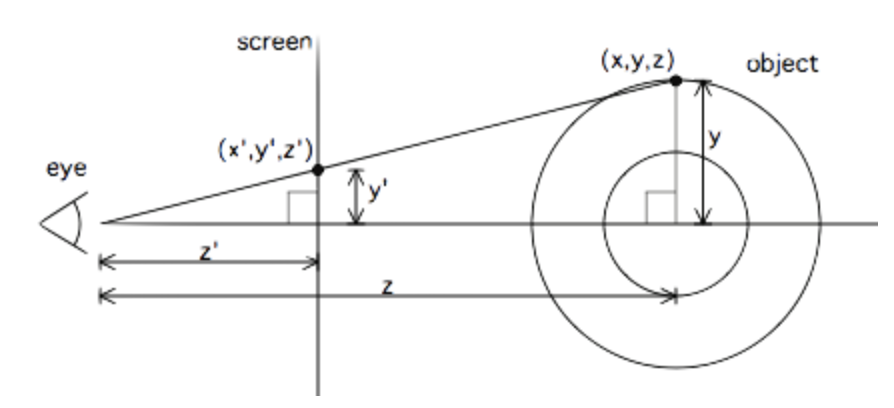
\includegraphics[width=0.5\linewidth]{Figures/projection.png}
        \label{fig1}
    \end{figure}

\end{frame}

%--------------------------------------------------------------------------------------------------

\section{Projection into terminal}
\begin{frame}
    \frametitle{z-buffer}

    As we mentioned before, when plotting a bunch of points, we might plot different points at the 
    same location but at different \emph{depths}, so we maintain a \emph{z-buffer}, which stores 
    the $z$ coordinate of everything we draw. If we need to plot a location, we first check whether 
    we're plotting in front of what's there already.

    \nullspace
    A trick to do this is by computing $z^{-1} = \frac{1}{z}$ and use that when depth buffering 
    because:
    \begin{itemize}
        \item $z^{-1} = 0$ corresponds to infinite depth, so we can initialize our z-buffer to 0 and 
            have the background be infinitely far away.
        \item We can re-use $z^{-1}$ when computing $x'$ and $y'$, since multiplication if much faster 
            than division.
    \end{itemize}

\end{frame}

%--------------------------------------------------------------------------------------------------

\section{Discrete Dynamic System}
\begin{frame}
    \frametitle{Discrete Dynamic System}

    Now, we are fully prepared to plot the result on the terminal. But one thing we need to be aware
    of is we can't really plot the 'animation', instead we plot frames one by one, which corresponding 
    to the concept to \emph{discrete dynamic system}. To be clearer, we have

    \begin{equation*}
        R(t + T) = R(t)
        \cdot
        \begin{pmatrix}
            x   \\
            y   \\
            z
        \end{pmatrix}
    \end{equation*}

    where $T$ is the time between two frames, $R(t)$ corresponds to all the linear transformation we 
    apply to a point.

\end{frame}

%--------------------------------------------------------------------------------------------------

\section{Discrete Dynamic System}
\begin{frame}
    \frametitle{Discrete Dynamic System}

    If we want to calculate a frame after a long time, we can actually \emph{diagonalize} $R(t)$
    as

    \begin{equation*}
        R(t) = S D(t) S^{-1}
    \end{equation*}
    where $S$ is the change of basis matrix for $R(t)$, $D(t)$ is a diagonal matrix whose diagonal 
    consists of \emph{eigenvalue} of $R(t)$.

    \nullspace
    Then we can quickly get $R^t(t)$ for large $n$ by
    
    \begin{equation*}
        R^n(t) = SD^n(t)S^{-1}
    \end{equation*}
    
    But in this case we actually need to calculate every frame, 
    so we do not need to change basis procedure.

\end{frame}

%--------------------------------------------------------------------------------------------------

\section{Demonstration}
\begin{frame}
    \frametitle{Demonstration}

    \begin{center}
        \animategraphics[autoplay,loop,width=8cm]{30}{Gifs/demo_donut/donut-}{0}{508}
    \end{center}
    

\end{frame}

%--------------------------------------------------------------------------------------------------

\section{Demonstration}
\begin{frame}
    \frametitle{Demonstration}

    \begin{center}
        \animategraphics[autoplay,loop,width=8cm]{30}{Gifs/demo_sphere/sphere-}{0}{94}
    \end{center}

\end{frame}

%--------------------------------------------------------------------------------------------------

\defverbatim[colored]\lstI{
    \begin{lstlisting}
                             k;double sin()
                         ,cos();main(){float A=
                       0,B=0,i,j,z[1760];char b[
                    1760];printf("\x1b[2J");for(;;)
                  {memset(b,32,1760);memset(z,0,7040)
                  ;for(j=0;6.28>j;j+=0.07)for(i=0;6.28
                 >i;i+=0.02){float c=sin(i),d=cos(j),e=
                 sin(A),f=sin(j),g=cos(A),h=d+2,D=1/(c*
                 h*e+f*g+5),l=cos      (i),m=cos(B),n=s\
                in(B),t=c*h*g-f*        e;int x=40+30*D*
                (l*h*m-t*n),y=            12+15*D*(l*h*n
                +t*m),o=x+80*y,          N=8*((f*e-c*d*g
                 )*m-c*d*e-f*g-l        *d*n);if(22>y&&
                 y>0&&x>0&&80>x&&D>z[o]){z[o]=D;;;b[o]=
                 ".,-~:;=!*#$@"[N>0?N:0];}}/*#****!!-*/
                  printf("\x1b[H");for(k=0;1761>k;k++)
                   putchar(k%80?b[k]:10);A+=0.04;B+=
                     0.02;}}/* To compile it ******
                      * gcc donut.c -lm -o donut *
                        ****** To run it *******
                            **** ./donut **/
    \end{lstlisting}
}

\section{Source Code}
\begin{frame}
    \frametitle{Source Code}

    \lstI

\end{frame}

%--------------------------------------------------------------------------------------------------

\section{Reference}
\begin{frame}
    \frametitle{Reference}

    \small{
        \begin{itemize}
            \item \url{https://www.a1k0n.net/2011/07/20/donut-math.html}
            \item \url{https://en.wikipedia.org/wiki/3D_computer_graphics}
            \item \url{https://www.javatpoint.com/computer-graphics-z-buffer-algorithm}
            \item \url{https://github.com/3b1b/manim}
        \end{itemize}
    }
    
\end{frame}


\end{document}
